\section{Background}

Classical molecular dynamics simulations were performed to analyze the interface formed between various aqueous salt solutions and carbontetrachloride. Three salt solutions were simulated, as well as a reference system consisting of neat water for comparison to previous computational efforts.\cite{Hore2007,Hore2008,Hore2007a,Walker2006b,Walker2007a,Walker2007b} The salts used in the simulations were NaCl, NaNO$_3$, and Na$_2$SO$_4$. These were chosen to compare to the experimental SFG results, and to supplement those experiments with additional molecular-level information. Analyses were performed on the simulation data to extract ionic and molecular density data, information about water coordination near to the interface, and water orientation data from order parameter analysis. The analyses are similar to, and logical extensions of previous computational work done on aqueous salt systems.

\subsection{Density Profiles}
Density histograms of simulated interfaces have been used in previous publications to show ionic and molecular distribution behavior in various systems.\cite{Chang1995,Eggimann2008,Du2008,Wick2006c,Petersen2005a,Hore2008,Walker2006b,Walker2007b} In this work the density profile of water through the interface is fitted to a hyperbolic tangent function\cite{Wick2006c,MATSUMOTO1988} as shown below:

\begin{equation}\label{tanh_fit}
	\rho(z) = \frac12(\rho_1+\rho_2) - \frac12\left(\rho_1-\rho_2\right)\tanh\left(\frac{z-z_0}{d}\right)
\end{equation}

Equation (\ref{tanh_fit}) relates the interfacial density, $\rho$, as a function of position, $z$, along a given system axis, to the densities of the phase on either side of the location of the Gibb's dividing surface, $z_0$. The bulk density $\rho_1$ and the density within the second phase, $\rho_2$ are fitted.  The interfacial width, $d$, is related to the ``90-10'' thickness of the interface by:

\begin{equation}\label{90-10}
	t = 2.197d
\end{equation}

These measures of interfacial thickness provide a means of comparing the depths to which the water phase is affected by ions located at the interface. The density distributions of the salts depict concentration and depletion phenomena throughout the interfacial region, and also serve to illustrate ionic affinity within this region. Previous work has been performed on the air-water interface with various ions introduced, showing varying levels of interfacial affinity, with the more polar ions being the most interfacially active. We present the density distribution results below for the neat-H$_2$O and salt solutions interfaced with an organic CCl$_4$ phase. %The density profiles of the different ionic species are fitted using a modified $\tanh()$ function that includes a gaussian function to more closely fit the concentration near the interface. The anion fitting function allows for a more direct comparison of location and peak width between the different systems.

%\begin{equation}\label{ion_fit}
	%\rho(z) = \frac12(\rho_1+\rho_2) - \frac12\left(\rho_1-\rho_2\right)\tanh\left(\frac{z-z_0}{d}\right) + ae^{-\frac{(x-b)^2}{2c^2}}
%\end{equation}

%The gaussian function allows one to locate the anion peak height $a$, centered at an offset location $b$, with a width $c$.

%\subsection{Water Coordination}
%The coordination of water and distribution of the various coordination types was determined for each intefacial system. Water coordination refers to the hydrogen-bonding structure of water molecules, and is a measure of the number and type of bonds made. A simple naming scheme used to describe each type of water coordination has been developed previously,\cite{Walker2006b} and so that nomenclature will be used in this work. It has been established that certain bonding structures dominate in different regions of the interface, thus each of the water density profiles will be broken down further into component coordination types to show the areas in which the various types are most prevalent. The parameters used to define a hydrogen-bond are taken from a previous work by this group.\cite{Walker2006b} Analysis of water coordination profiles is valuable for comparison to experimental VSF results within the OH-bond stretching region of the vibrational spectrum. These give a molecular-level description of the composition of an interface, and show the various water bonding types that will contribute most to the VSF signal. Additionally, the results of this work are compared to previous studies on the air and salt water interfaces to establish differences due to the addition of the CCl$_4$ organic phase.

%\subsection{Order Parameters}
%One means of describing molecular orientation near to interfaces is by use of orientational order parameters.\cite{Buffeteau2004} This technique has been applied to biaxial molecules such as water at organic interfaces,\cite{Hore2008} and organic molecules to elucidate structuring within the interfacial region.\cite{Hore2007} In this work we compute the two order parameters, S$_1$ and S$_2$, as functions of distance from the Gibbs dividing surface.

%\begin{equation}\label{s1 parameter}
	%S_1 = \frac12\left<3 \cos^2(\theta) - 1\right>
%\end{equation}
%
%\begin{equation}\label{s2 parameter}
	%S_2 = \frac{\left<\sin(\theta)\cos(2\phi)\right>}{\left<\sin(\theta)\right>}
%\end{equation}

%The order parameters are calculated from the euler angle values of the molecular ``tilt'' $\theta$, and the ``twist'' $\phi$. %The order parameter distributions are further broken down to show the values for individual water coordination types for determination of orientational behavior of each.

\subsection{Molecular Orientation}
% Describe method used to find the bisector and normal orientation histograms
Several methods have been used previously to show molecular orientation profiles of water molecules throughout simulated interfacial regions.\cite{Someone} In this work we have chosen to compute the orientation of water using two vectors that fully describe the orientation in space given the locations of the three atoms comprising the molecule. The molecular bisector, a vector that points along the axis of symmetry of the water molecule from the hydrogen-end to the oxygen, provides directional orientation of the molecule in an intuitive way. A second vector, what is refered to here as the molecular normal vector, is established as the vector pointing normal to the plane formed by the three atoms of the water molecule and establishes the ``tilt'' of the molecule. Analyzing the angle made between these two vectors and a given space-fixed axis (the long axis of the system) is a means of finding the absolute orientation of waters within these simulated systems as illustrated in figure \ref{fig:water-angles}. The angle between the molecular bisector and the system $Z$-axis will hereafter be referred to as $\theta$, and the molecular normal vector as $\phi$. The analysis in this work reports the cosines of these two angles, and because of the symmetry of the water molecule where the hydrogens are not uniquely identified, the cosines of the two angles are limited as follows: $-1\le\theta\le1$ and $0\le\phi\le1$. We report here two-dimensional histograms showing the orientation profiles of $\theta$ and $\phi$ as functions of the distance from the gibbs dividing surface of the interface, as found from the fitting in our density profile analyses.

\begin{figure}[h!]
\begin{center}
	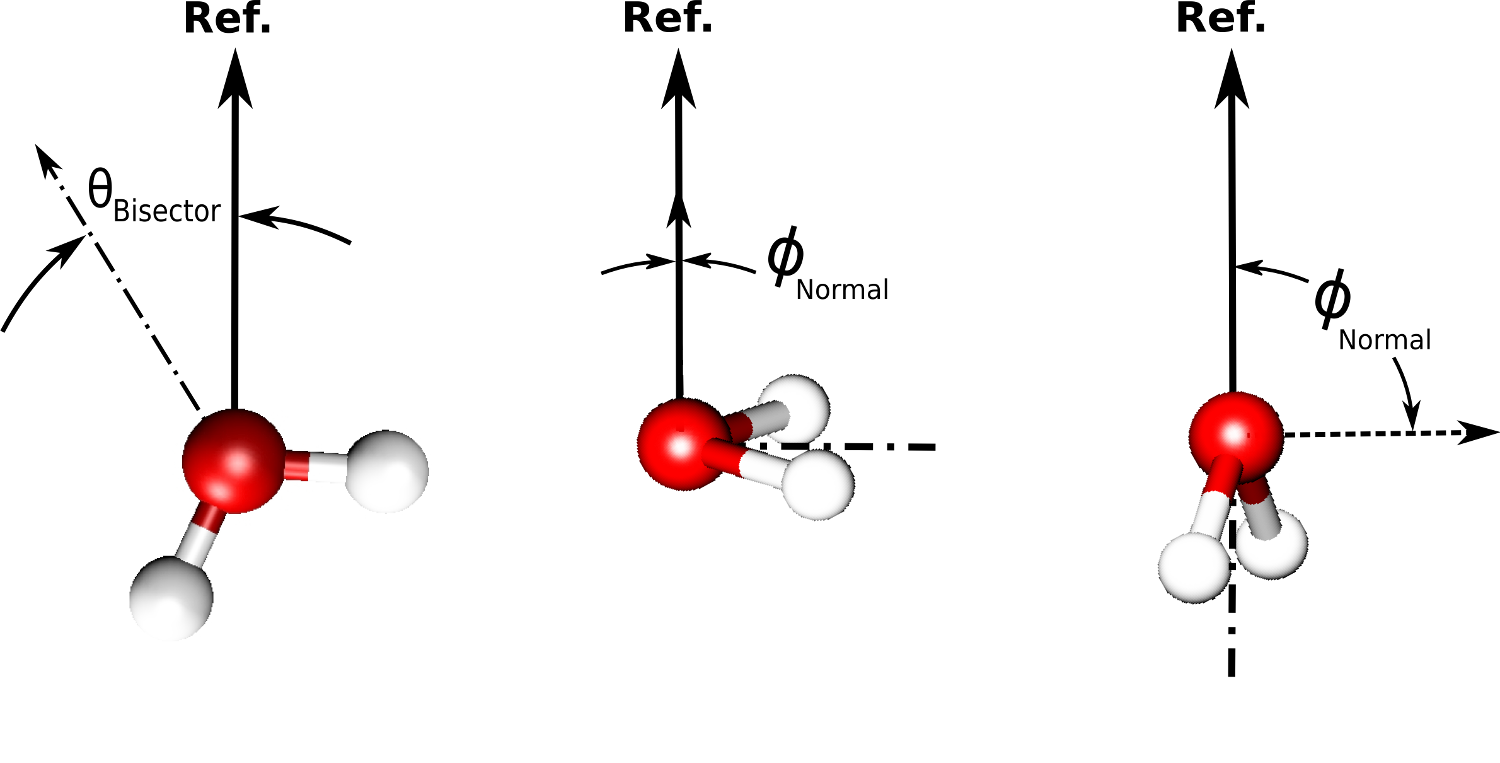
\includegraphics[scale=0.3]{images/water-angles.png}
	\caption{Angles used to define molecular orientation. The system reference axis (i.e. the system Z-axis) is that which is perpendicular to the plane of the aqueous-organic interface, and points out from the aqueous phase into the organic one. The molecular bisector vector points from the hydrogen-end of the water to the oxygen end, and orients along the axis of symmetry. The angle it forms with the reference axis is either aligned or anti-aligned such that $-1\le \cos(\theta) \le 1$. The angle formed between the vector normal to the molecular plane (formed by the three water atoms) and the reference-axis orients the ``twist'' of the molecule such that $0 \le \cos(\phi) \le 1$, where the water molecular plane is either laying flat on the interface ($\cos(\phi)=1$) or it the water is perpendicular to the interface ($\cos(\phi)=0$).}
	\label{fig:water-angles}
\end{center}
\end{figure}

%\begin{figure}[h!]
%\begin{center}
%	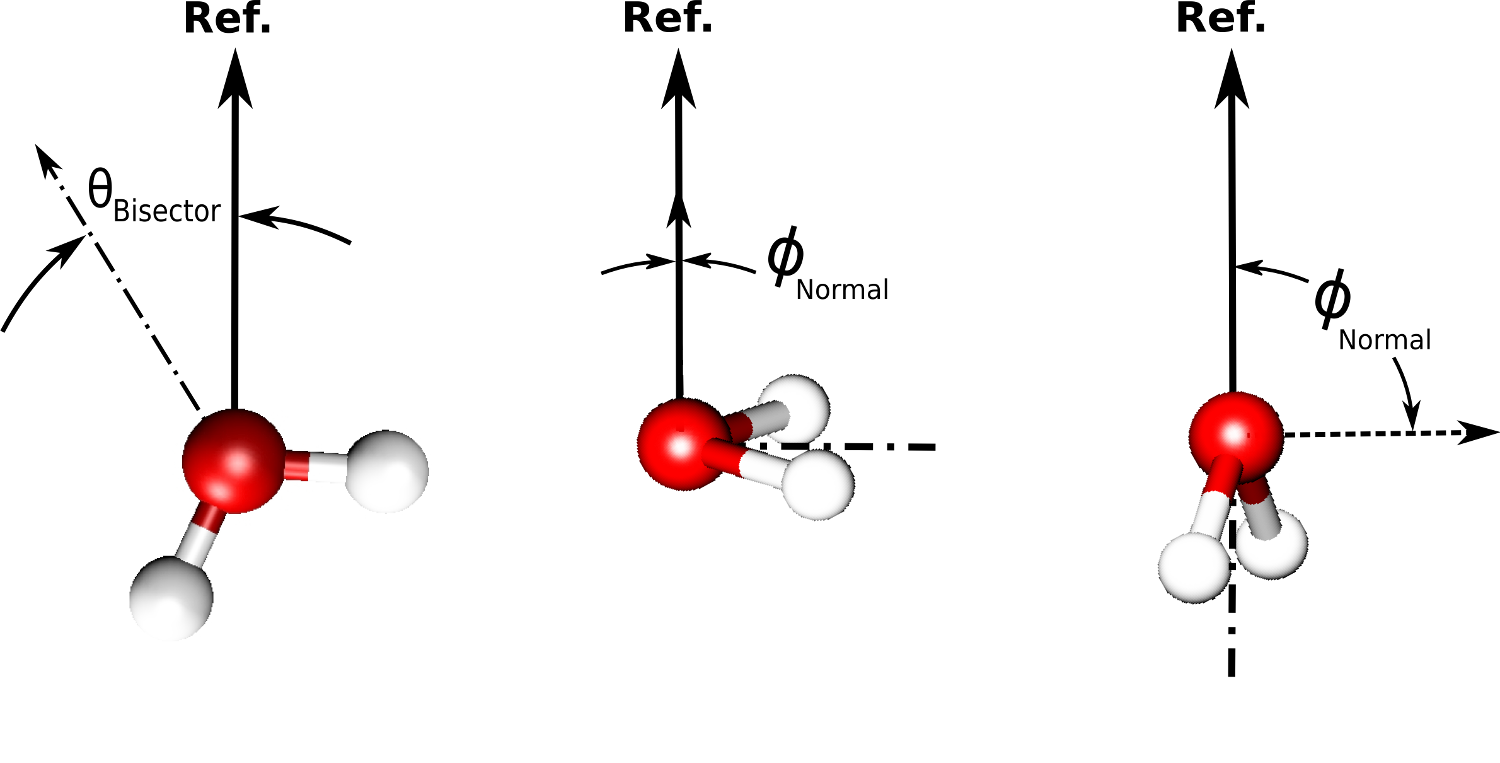
\includegraphics[scale=1.0]{images/water-angles.png}
%	\caption{Molecular orientation of water molecules. The system axis perpendicular to the aqueous interface is used as a reference for analysis of molecular orientation. The angle formed between the reference axis and the water molecular bisector vector, $\theta$, may vary such that $-1<\cos(\theta)<1$. When $\cos(\theta)$ is 1, the molecule's bisector is perfectly aligned with the reference axis, and $\cos(\theta)=-1$ results from a perfect anti-alignment. A second angle, $\phi$, describes the molecular ``twist'' about the bisector. The symmetry of the water molecule limits the range of $\phi$ to $0<cos(\phi)<1$. $\cos(\phi)=0$ results from a water that lies with its molecular plane perpendicular to the plane of the interface, and $\cos(\phi)=1$ describes a water lying perfectly parallel to the plane of the interface.
%	\label{fig:water-angles}
%\end{center}
%\end{figure}


%insert graphic showing bisector and water-plane normal vectors relative to the system Z-axis

\subsection{Radial Distribution Functions}

In studying the water structure near to the interface with an organic phase, the radial distribution functions (RDF) for the water atoms were computed lending another metric of water's structure. The RDF's, $g(r)$, for each system were calculated and normalized to a gas-phase probability of unity at long distances, representing a complete loss of orientational correlation.

\subsection{Computational SFG}
%Describe SFG computational method
A difficult challenge for experimental surface studies is in understanding the vibrational spectroscopy of liquid water. Hydrogen bonding between water molecules causes intermolecular and intramolecular couplings. Simulations provide the the analytical capacity to relate the broad lineshapes, and the often difficultly assessed impact of hydrogen bonding as a function of OH vibrational frequency, to microscopic geometries, forces, and environments. In this work we compute the SFG spectra of the interface between the salt solutions and an orgnanic phase to qualify the conclusions of a previous experimental work by our group\cite{McFearin2009} and to elucidate some of the microscopic phenomena that lead to spectroscopic signatures.

The computational method used in this work is based on that of Morita and Hynes\cite{Morita2000} as outlined in a previous study by this group utilizing the same technique.\cite{Walker2007} The computational SFG technique has been improved in more recent studies by Morita et al,\cite{Morita2002,Ishiyama2009} and with other enhanced water models. The technique used in this work has been established to recreate the qualities of the experimental spectra to a sufficient degree such that we may still draw qualified conclusions about lineshape and intensity. The most dramatic short-coming of the current technique is that of reproducing the lower-frequency features of the SFG spectra below the 3200 cm$^-1$ region. However, our present analysis is concerned primarily with the overall intensity and response, and thus we still draw qualitative conclusions based on our computed results, and utilize the simpler computational methods from our previous works.
